\chapter{Влияние рассеяния носителей на шероховатой поверхности на оптические свойства размерно-ограниченных систем} \label{chapt2}

\section{Межподзонное и внутризонное поглощение света в квантовых системах с пониженной размерностью с учетом рассеяния на шероховатой поверхности} \label{sect2_1}

В наноструктурах зона проводимости (как и валентная зона) квантуется, поэтому возникают новые каналы поглощения (излучения) слабой электромагнитной волны в далекой инфракрасной области спектра, связанные с переходом электрона между размерно-квантованными состояниями зоны проводимости (рисунок~\ref{img:fig_2_1_1}).  В работе \cite{West1985} впервые наблюдалось такое поглощение света в квантовых ямах $\text{GaAs}/\text{Al}_{0.30}\text{Ga}_{0.7}\text{As}$ с толщинами $65 \AA$ и $82 \AA$ (переход I на рисунок~\ref{img:fig_2_1_1}). Как показали экспериментальные исследования, частотная зависимость коэффициента поглощения света хорошо описывается лоренцовской кривой, и полуширина линии поглощения при комнатных температурах $\cong 10 \text{ meV}$, что может быть связано со взаимодействием электрона с фононами. В работах \cite{Wu1994,Spector1983} исследовалось поглощение света свободными носителями в широких $(a > 10^3 \AA)$ квазидвумерных полупроводниковых структурах в нижайшем порядке теории возмущений по взаимодействию электронов с длинноволновыми акустическими колебаниями. В частности показано, что коэффициент поглощения света с ростом ширины квантовой системы уменьшается и с ростом температуры увеличивается. Однако в узких нелегированных размерно-ограниченных системах при низких температурах возможным и наиболее важным является рассеяние носителей на шероховатой поверхности. Этот механизм рассеяния определяет величину и температурную зависимость подвижности в квантовых ямах \cite{Sakaki1987}, в кремниевых инверсионных слоях \cite{Stern1980}, в которых электронный газ остается вырожденным вплоть до $T < 100 K$. Влияние шероховатой поверхности на процессы фотолюминесценции в узких $(a \geq 50 \AA)$ одиночных квантовых ямах GaAs/AlGaAs  проводилось в \cite{Gurioli1991} при $T = 4 K$. Теоретические исследования поглощения света свободными носителями с учетом взаимодействия электрона с шероховатой поверхностью проводились в \cite{Vurgaftman1999}. Рассматривался, как случай поглощения света ТМ–поляризации (электромагнитная волна распространяется вдоль оси пространственного квантования), так и случай поглощения ТЕ-поляризации (электромагнитная волна распространяется нормально к поверхности квантовой системы). В обоих случаях коэффициент поглощения света рассчитывался в нижайшем порядке по взаимодействию электрона с шероховатой поверхностью. Численные расчеты для коэффициента поглощения света справедливы естественно для частот электромагнитной волны вдали от максимума поглощения (для ТМ-поляризованной волны) и при малых взаимодействиях электрона с поверхностью исследуемой квантовой системы.

\begin{figure}[!h] 
	\center
	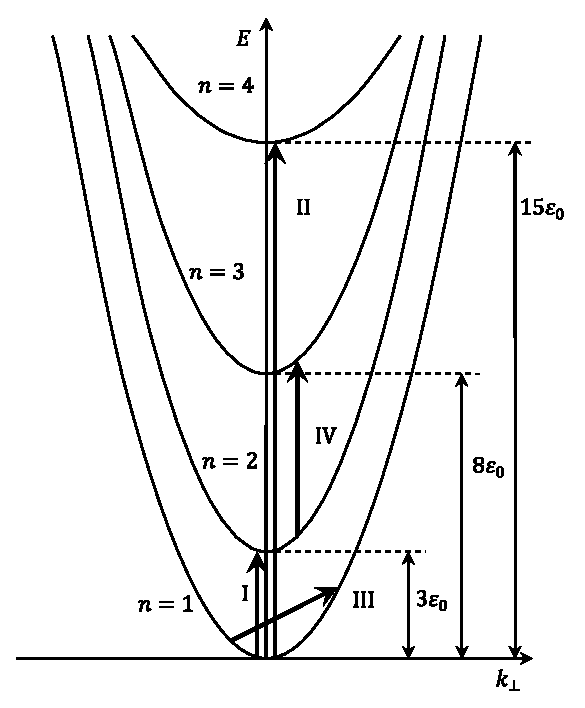
\includegraphics [scale=1] {fig_2_1_1}
	\caption{Энергетическая диаграмма для размерно-квантованной зоны проводимости в размерно-ограниченных системах. Стрелками указаны возможные оптические переходы.} 
	\label{img:fig_2_1_1} 
\end{figure}

В работах \cite{Aleshkin2002,Vorobiev2004} экспериментально, а в \cite{Thammasat1997} теоретически исследовалось межзонное поглощение света в ступенчатых квантовых ямах InGaAs/AlGaAs. При высоких уровнях возбуждения заполняются, как основная подзона, так и возбужденные состояния, что позволило наблюдать поглощение инфракрасного излучения, связанного с переходами электрона между возбужденными состояниями (переход IV на рисунке~\ref{img:fig_2_1_1}). При этом коэффициент поглощения достигает больших значений $(\sim 10^3 \text{ cm}^{-1})$ при высоких температурах $T \simeq 300^{\circ}K$. Влияние поверхности на оптические характеристики в квантовых ямах GaAs/AlGaAs экспериментально исследовалось в \cite{Gurioli1991,Weisbuch1981}. В частности было показано, что учет шероховатой поверхности приводит к уширению спектров фотолюминесценции.

Далее проводится расчет коэффициента поглощения слабой электромагнитной волны $K\left(\Omega \right)$ различной поляризации, как для внутризонных переходов (переход III на рисунке~\ref{img:fig_2_1_1}), так и для межподзонных переходов (переходы I, II) с учетом взаимодействия электронов с шероховатой поверхностью в квантовой яме. При этом коэффициент поглощения электромагнитной волны вычисляется без использования теории возмущений по взаимодействию носителей с шероховатой поверхностью, как это делалось в \cite{Vurgaftman1999}, что позволяет исследовать частотную зависимость $K(\Omega)$ в широкой области частот и сформулировать условия применимости теории возмущений и последовательно описать внутризонное поглощение света и при неслабых взаимодействиях электрона с шероховатой поверхностью.	

Расчет коэффициента поглощения света частоты $\Omega$ и вектора поляризации $\vect{\xi}$ проводится по формуле Кубо \cite{Kubo1957a}, которая в представлении вторичного квантования имеет вид \cite{Sinyavskii2010}:
\begin{multline} \label{eq:21_02}
K(\Omega) = \frac{2 \pi e^2}{V c n_0 \hbar \Omega m_e^2}\left( 1 - e^{-\beta_0 \hbar \Omega} \right) \sum_{\alpha \alpha_1 \beta \beta_1} {\left\langle \alpha \left| (\hat{\vect{P}} \vect{\xi})  \right| \alpha_1 \right\rangle \left\langle \beta \left| (\hat{\vect{P}} \vect{\xi})  \right| \beta_1 \right\rangle} \times\\
\times\int\limits_{-\infty }^{\infty} {dt e^{i\Omega t}\left\langle a_{\alpha }^+ (t) a_{\alpha_1 }(t) a_{\beta }^+ a_{\beta_1 } \right\rangle}  ,
\end{multline} 
${\left| \alpha  \right\rangle} $~---~волновые функции свободного электрона,   $a_{\alpha}^+ (a_{\alpha})$~---~операторы рождения (уничтожения) электрона с эффективной массой $m_e$ в состоянии $\alpha$,  $n_0$~---~показатель преломления, $V$~---~объем основной области квантовой системы,  $\hat{\vect{P}}$~---~оператор импульса, $\beta_0 = 1 / T$,  $T$~---~температура,
\[
a_{\alpha }^+ (t)= \exp\left(\frac{it\hat{H}}{\hbar } \right)a_{\alpha }^+ \exp\left(-\frac{it\hat{H}}{\hbar } \right), \;
\hat{H} = \hat{H}_0 + V, \;
\hat{H}_0 {\left| \alpha  \right\rangle} = E_{\alpha} {\left| \alpha  \right\rangle}.
\]
$V$~---~описывает взаимодействие электрона с шероховатой поверхностью исследуемой наноструктуры шириной $a$ \eqref{eq:1_1}.

Если учесть, что временная зависимость операторов рождения и уничтожения определяется соотношениями \cite{Khamidullin2002}:
\begin{equation} \label{eq:21_04}
a_{\alpha}^+ (t) = \sum_{\gamma}{a_{\gamma}^+ \left\langle \gamma \left| \exp{\left( \frac{it\widetilde{H}}{\hbar}\right) } \right| \alpha \right\rangle},
\end{equation}
\begin{equation} \label{eq:21_06}
a_{\alpha} (t) = \sum_{\gamma}{\left\langle \alpha \left| \exp{\left(- \frac{it\widetilde{H}}{\hbar}\right) } \right| \gamma \right\rangle a_{\gamma}},
\end{equation}  
($\widetilde{H}$~---~гамильтониан рассматриваемой задачи в координатном представлении), то после подстановки \eqref{eq:21_04}, \eqref{eq:21_06} в \eqref{eq:21_02} не трудно получить следующее выражение для коэффициента поглощения слабой электромагнитной волны: 
\begin{multline} \label{eq:21_08}
K(\Omega) = \frac{2 \pi e^2 }{V c n_0 \hbar \Omega m_e^2}\left( 1 - e^{-\beta_0 \hbar \Omega} \right) \int\limits_{-\infty }^{\infty} {dt \sum_{\alpha \alpha_1 \beta \beta_1} {\left\langle \alpha \left| (\hat{\vect{P}} \vect{\xi})  \right| \alpha_1 \right\rangle \left\langle \beta \left| (\hat{\vect{P}} \vect{\xi})  \right| \beta_1 \right\rangle}} \times\\
\times n_{\beta_1} \left(1-n_{\beta} \right)
{\left\lbrace  \left\langle \beta_1 \left| \exp \left(\frac{it\widetilde{H}}{\hbar}\right) \right|\alpha\right\rangle \left\langle \alpha_1 \left| \exp \left(-\frac{it\widetilde{H}}{\hbar}\right) \right|\beta\right\rangle \right\rbrace }_V  .
\end{multline} 
При записи \eqref{eq:21_08} было проведено усреднение по системе свободных электронов; $n_\alpha = \left\{ \exp\left[ \beta \left( \varepsilon _\alpha - \xi \right) \right] + 1 \right\}^{- 1}$~---~равновесная
функция распределения для электронов с энергией $\varepsilon{_\alpha}$, $\xi $~---~химический потенциал.

Не трудно показать, что для прямоугольной квантовой ямы матричные элементы оператора импульса определяются соотношениями $(\alpha (n, \vect{k}{_\bot}), \; \beta (n', \vect{k}'_{\bot}))$:
\begin{equation} \label{eq:21_09_01}
\left\langle \alpha \left| \hat{p}^{(z)} \right| \beta \right\rangle = \frac{2}{a} i\hbar \delta_{k_\bot k'_\bot} \frac{n n_1}{n^2 - n_1^2} \left[(-1)^{n+n_1} -1 \right] , \; n \neq n_1
\end{equation}
\begin{equation} \label{eq:21_09_02}
\left\langle \alpha \left| \hat{p}^{(x)} \right| \beta \right\rangle = \hbar k_x \delta_{\alpha\beta},\;
\left\langle \alpha \left| \hat{p}^{(y)} \right| \beta \right\rangle = \hbar k_y \delta_{\alpha\beta}.
\end{equation} 

Как непосредственно следует из \eqref{eq:21_09_01}, \eqref{eq:21_09_02} поглощение света, связанное с переходами электрона между размерно-квантованными зонами проводимости $n \neq n_1$  (переходы I, II, IV на рисунке~\ref{img:fig_2_1_1}), возможно только в ТМ–поляризации \eqref{eq:21_09_01}. Будем предполагать, что рассеяние электронов на шероховатой поверхности для различных размерно-квантованных зон, между которыми происходит оптический переход, происходит независимо. Усреднение в \eqref{eq:21_08} по реализации случайного процесса проведём с использованием кумулянтного усреднения \cite{Kubo1962}. С точностью до второй кумулянты получаем:
\begin{multline} \label{eq:21_09_04}
I = {\left\lbrace  \left\langle \beta_1 \left| \exp \left(\frac{it\hat{H}}{\hbar}\right) \right|\alpha\right\rangle \left\langle \alpha_1 \left| \exp \left(-\frac{it\hat{H}}{\hbar}\right) \right|\beta\right\rangle \right\rbrace }_V \approx \\
\approx \delta_{\beta_1\alpha} \delta_{\alpha_1\beta} \exp{\left[\frac{it}{\hbar} \left(E_{\alpha} - E_{\alpha_1} \right)  \right] } \exp{\left[- g_{\alpha\alpha_1}(t) \right]}
\end{multline} 
\begin{multline} \label{21_09_06}
g_{\alpha\alpha_1 }(t)=\frac{1}{{\hbar }^2}\int\limits_0^t d \tau \int\limits_0^{\tau }d \tau_1 \sum_{\gamma} \left\{ W_{\alpha\gamma }\exp \left[\frac{i}{\hbar }\left(\tau_1-\tau \right) \left(E_{\alpha}-E_{\gamma }\right)\right] + \right.\\
\left. + W_{\alpha_1\gamma} \exp \left[\frac{i}{\hbar }\left(\tau_1-\tau \right)\left(E_{\alpha_1}-E_{\gamma }\right)\right] \right\}
\end{multline} 

В результате, если использовать приближение времени релаксации \eqref{eq:31_130}, и пренебречь поправками к энергии свободных электронов, связанными с рассеяниями носителей на шероховатой поверхности, не трудно получить:
\begin{equation} \label{eq:21_09_08}
I = \delta_{\beta_1\alpha} \delta_{\alpha_1\beta} \exp{\left[\frac{it}{\hbar} \left(\widetilde{E}_{\alpha} - \widetilde{E}_{\alpha_1} \right)  \right] } \exp{\left(- \frac{|t|}{\tau_{\alpha\alpha_1}} \right)}.
\end{equation}
Здесь введены следующие обозначения:
\[
\widetilde{E}_{\alpha} = E_{\alpha} - \frac{W_{\alpha \gamma}}{E_{\alpha} - E_{\gamma}}
\]
\[
W_{\alpha\beta}=\int{d\vect{r} d\vect{r_1} \Psi^*_\alpha(\vect{r}) \Psi^*_\beta(\vect{r_1}) V_\alpha V_\beta F \Psi_\alpha(\vect{r_1}) \Psi_\beta(\vect{r})}
\]
\[
\frac{1}{\tau_{\alpha\alpha_1}} = \frac{\pi}{\hbar} \sum_{\gamma } { \left[W_{\alpha \gamma }\delta \left(E_{\alpha} - E_{\gamma}\right) + W_{\alpha_1 \gamma }\delta \left(E_{\alpha_1} - E_{\gamma}\right) \right] }
\]
Для случая $\delta$-коррелированной флуктуации поверхности
\begin{equation} \label{eq:21_09_10}
\frac{1}{\tau_{\alpha\alpha_1}} = \frac{1}{\tau_0} \left(n^4 + n_1^4 \right) ,
\end{equation}
\[
\frac{1}{\tau_0}  = \frac{m_e}{2\hbar^3} \left(\frac{2\varepsilon_0}{a} \right)^2 \gamma_0. 
\]
Из \eqref{eq:21_09_10} следует, что время релаксации при рассеянии носителей на шероховатой поверхности не зависит от волнового вектора электрона и заметным образом уменьшается с ростом $n$ и $n_1$. Для невырожденного электронного газа, если использовать соотношения \eqref{eq:21_08} и \eqref{eq:21_09_10}, то коэффициент поглощения света, связанный с переходом электрона из нижайшей зоны проводимости $(n=1)$ в ближайшую размерно-квантованную зону проводимости $(n_1=2)$ (переход I на рисунке~\ref{img:fig_2_1_1}), записывается следующим образом $(\beta _0\hbar \Omega \gg 1)$:
\begin{equation} \label{eq:21_10}
K(\Omega) = K_M \frac{1}{1+\left(\dfrac{\tau_0 }{17 \hbar} \Delta_0 \right)^2 } ;
\end{equation} 
\[
K_M =\frac{2^{12} e^2 a^5 n_e }{\hbar cn_0 \pi^5 \gamma_0 3^3 \cdot 17}, \;
\Delta_0 =\hbar \Omega -3\varepsilon_0.
\]
$n_e =N/L_x L_y $~---~поверхностная плотность электронов. При записи (\ref{eq:21_10}) учитывалось, что в размерно-квантованной зоне, на которую происходит оптический переход носителя, электронов нет, поэтому $n_{\beta } \ll 1$. Последнее приближение вполне справедливо, если  $3\varepsilon_0 \gg kT$, т.е. почти все электроны находятся на нижайшей размерно-квантованной зоне проводимости $(n=1)$, и, следовательно, $\sum n_{k_{\bot } } \cong N$ ($N$~---~число электронов в исследуемой квантовой системе). Из \eqref{eq:21_10} следует, что частотная зависимость коэффициента поглощения света описывается лоренцовой кривой с полушириной  $\delta =17\cdot 2\hbar /\tau_0 $. Величина коэффициента поглощения электромагнитной волны при рассматриваемом механизме рассеяния существенным образом определяется толщиной квантовой ямы $\left(K_M \sim a^5 \right)$ и не зависит от температуры. $K\left(\Omega \right)$  в максимуме при $n_e =4\cdot 10^{11} \text{cm}^{-2} $, $n_0 = 3.2$,   принимает значение   $K_M^{\left(\delta \right)} =0.25\cdot a_0^5 /\gamma_0 $ ($a_0 $, $\sqrt[4]{\gamma_0}$~--–~измеряются в ангстремах), т.е. при  $a_0 = 80 \AA$,  $\sqrt[4]{\gamma_0} = 10 \AA$ (именно такие значения   хорошо описывают значения подвижности   экспериментально наблюдаемые в КЯ GaAs/AlGaAs \cite{West1985}), $K_M =2\cdot 10^4 \text{cm}^{-1} $. Большие значения коэффициента поглощения света позволяют надеяться на практическое использование таких размерно-квантованных систем в качестве детекторов ИК-излучения в области низких температур. Полуширина линии поглощения для рассматриваемого прямого оптического перехода при рассматриваемых выше параметрах $\delta =6.5\cdot 10^6 \left(\gamma_0 /a_0^6 \right)\text{meV}$. Следовательно, при  $a_0 = 60 \AA$,  $\sqrt[4]{\gamma_0} = 15 \AA$,  $\delta = 7 \text{ meV}$, что безусловно, находится в области экспериментального измерения.

Для ТЕ-поляризованного излучения, из \eqref{eq:21_09_02} следует, что  возможно поглощение света только в одной размерно-квантованной зоне проводимости (переход III на рисунке~\ref{img:fig_2_1_1}). В этом случае функция \eqref{21_09_06} после интегрирования по $\tau$ и $\tau_1$ может быть записана следующим образом:
\begin{equation} \label{eq:21_09_12}
g_{\alpha\alpha_1 }(t) =2 \sum_{\gamma}  \frac{ W_{\alpha\gamma }}{\left(E_{\alpha} - E_{\gamma} \right)^2 } \left[1 - \cos{\frac{t}{\hbar} \left( E_{\alpha} - E_{\gamma} \right) } \right] .
\end{equation}

Рассмотрим поглощение слабой электромагнитной волны в нижайшей $(n=1)$ размерно-квантованной зоне. Если провести суммирование в \eqref{eq:21_09_12} по $\gamma$ $\left( E_{\gamma} = \varepsilon_0 + \hbar^2 {k'}_{\bot}^2 / {2m_e} \right) $ и подставить $g_{\alpha\alpha_1 }(t)$ в \eqref{eq:21_08}, то выражение для коэффициента поглощения света в случае невырожденного электронного газа принимает вид:
\begin{multline} \label{21_09_14}
K(\Omega) = \frac{2 \pi e^2 n_e }{m_e c n_0 a \hbar \beta_0 \Omega^2} \int\limits_0^{\infty}x dx \int\limits_{-\infty}^{\infty}y dy \times \\
\times \exp{\left\lbrace  - 2\Gamma_0 |y| \left[ 1 - \frac{\delta_0}{\pi x |y|}\sin^2{\left( \frac{x|y|}{\delta_0}\right) } + \frac{1}{\pi} \mathrm{Si}{\left( \frac{2x|y|}{\delta_0}\right) } \right]  \right\rbrace   }.
\end{multline} 
Здесь введены следующие обозначения:
\[
\delta_0 = 2\hbar \Omega \beta_0,
\]
\[
\Gamma_0 = \pi^2 \left(\frac{\varepsilon_0}{\hbar \Omega} \right) \left( \frac{\gamma_0}{a^4} \right),
\]
\[
\mathrm{Si}(z) = -\frac{\pi}{2} + \int\limits_0^z{d\tau\frac{\sin{t}}{\tau}}.
\]

В случае низких температур выражение для поглощения света \eqref{21_09_14} можно записать:
\begin{equation} \label{eq:21_20}
K(\Omega )=\frac{4\pi e^{2} n_{e} }{m_e c n_0 a \hbar\beta \Omega^2 } \frac{\Gamma_0 }{1+\Gamma_0^2 }
\end{equation} 

Как показывают численные расчеты, соотношение \ref{eq:21_20} при больших $\delta_0$ мало отличается от точного \ref{eq:21_20}. Например, при $\delta_0 > 5$ отличие менее 10\% в широком интервале изменения $\Gamma_0$. Заметим, что в нижайшем приближении по взаимодействию электрона с шероховатой поверхностью $\Gamma_0 \ll 1$, что соответствует обычной теории возмущений, тогда из (\ref{eq:21_20}) нетрудно получить:
\begin{equation} \label{eq:21_30}
K(\Omega )=\frac{2^4 e^2 n_e \gamma_0 m}{\pi c n_0 a\hbar^3 \beta_0 } \left(\frac{\varepsilon_0 }{\hbar\Omega } \right)^3
\end{equation} 

В рассматриваемом случае $K(\Omega )\sim \Omega^{-3} $ и при низких температурах ($T=50 K$) для $\gamma_0^{1/4} =15 \AA$, $n_e = 2\cdot 10^{12} \text{cm}^{-2} $, $a=50 \AA$, $K_0 (\Omega )\cong 10\left(\varepsilon_0 / \hbar\Omega \right)^3 \text{cm}^{-1} $.

При $\Gamma_0 \gg 1$, что соответствует сильному взаимодействию электрона с шероховатой поверхностью, коэффициент внутризонного поглощения электромагнитной волны определяется соотношением:
\begin{equation} \label{eq:21_40}
K(\Omega )=\frac{2^4 e^2 n_e a}{\pi^3 cn_0 \hbar } \frac{1}{\delta_0 } \left(\frac{a^4 }{\gamma_0 } \right)
\end{equation} 

В рассматриваемом приближении сильной связи $a^4 /\gamma_0 =1$, $K(\Omega )\sim \Omega ^{-1} $ и для $\delta_0 =10$, $a=50 \AA$, $K(\Omega )\cong 120 \text{ cm}^{-1} $. Следовательно, в области низких частот для узких квантовых ям с большой флуктуацией поверхности теория возмущений при исследовании внутризонного поглощения света может оказаться несправедливой.
	

\section{Влияние лазерного излучения на оптические свойства квантовых пленок} \label{sect2_2}

Исследования резонансных явлений в физике твердого тела являются довольно привлекательными, так как в этом случае лазерное излучение приводит к заметному влиянию на кинетические явления даже при небольших интенсивностях электромагнитной волны. Примером может служить влияние инфракрасного (ИК) лазерного излучения частоты $\omega $ на коэффициент межзонного магнетопоглощения слабого света, когда $\omega $ равна циклотронной частоте $\omega_c $ (магнитоинфракрасный резонанс -- МИКР). В этом случае резонансное ИК-излучение оказывается причиной нестационарности электронных состояний и может полностью определять форму пиков магнетопоглощения слабой электромагнитной волны при небольших интенсивностях лазерного излучения. Наиболее ярко резонансные эффекты в кинетических коэффициентах могут проявляться в размерно-квантованных системах (параболические квантовые ямы), когда частота ИК лазерного излучения равна частоте размерного квантования (размерно-инфракрасный резонанс -- РИР). В частности, экспериментальное обнаружение влияния РИР на межзонное поглощение слабого света позволит не только обосновать используемые модели, но и говорить о совершенстве этих размерно-квантованных систем. В этом параграфе исследуется влияние постоянного электрического поля на межзонное поглощение слабой электромагнитной волны в режиме МИКР и РИР. Именно в постоянном электрическом поле, во-первых, наиболее отчетливо проявляются эффекты влияния на коэффициент поглощения света резонансного лазерного излучения и, во-вторых, возникают дополнительные особенности в высокочастотной области спектра поглощаемой электромагнитной волны.

Если магнитное поле $\vect{H}||OZ$, электрическое поле направлено вдоль $\vect{H}$, то гамильтониан для электрона в калибровке Ландау $A(-Hy,0,0)$ в поле лазерного излучения примет вид:

\begin{multline} \label{eq:22_10} 
\hat{H}_c =\frac{1}{2m_c } \hat{P}^2 +\frac{e}{m_e c} (\hat{P}\xi )\sqrt{\frac{4\pi c^2 }{V} } (\hat{b}+\hat{b}^+ ) + \\ 
+\frac{e^{2} }{2m_e c^2 } \left(\frac{4\pi c^{2} }{V} \right)(\hat{b}+\hat{b}^+ )^2 +\hbar \omega \hat{b}^+ \hat{b}+eEz\equiv \hat{H}_c^0 +eEz,
\end{multline}
где $\hat{P}=\hat{p}+\frac{e}{c} \hat{A}$; $\hat{b}^+ (\hat{b})$~---~операторы рождения (уничтожения) для интенсивного лазерного излучения частоты $\omega $, поляризации $\xi $; $V$~---~объем основной области кристалла; $m_e $~---~эффективная масса электрона.

Коэффициент межзонного поглощения слабой электромагнитной волны частоты $\Omega $ и поляризации $\xi _{0} $ согласно формуле Кубо \cite{Kubo1957a} можно привести к виду \cite{Sokovnich2004}:
\begin{multline} \label{eq:22_20} 
K(\Omega )=\frac{4\pi e^2 }{V n_0 c\hbar \Omega } \left|\frac{p_{cv} \xi_0 }{m_0 } \right|^2 \times  \\
\times \sum _{\beta } \int\limits_{-\infty }^{\infty} dt \exp \left(i\Omega t-\frac{i e^2 E^2 t^3 }{6\hbar \mu } +\frac{ieEk_z t^2}{2\mu } \right)\times  \\ 
\times \left\{<\beta^c |\exp \left(\frac{it}{\hbar } \hat{H}_v^0 \right)\exp \left(-\frac{it}{\hbar } \hat{H}_c^0 \right)|\beta^c >\right\}_f  
\end{multline} 
где $|\beta^c >$~---~волновые функции для электронов в зоне проводимости в отсутствии электрического поля; $\beta $~---~набор квантовых чисел, описывающих состояние заряженной частицы; $p_{cv} $~---~матричный элемент оператора импульса на блоховских функциях, $\mathop{\hat{H}}\nolimits_i^0 $~---~гамильтониан для электронов в магнитном поле в $i$-ой зоне ($i=c,v$); $\{ \}_f$~---~описывает усреднение по системе свободного фотонного поля \cite{Glauber1963,Klauder1968}. 

Далее исследуем случай, когда электрическое поле $\vect{E_0} $ линейно-поляризованного лазерного излучения перпендикулярно $\vect{H}$, т.е. лазерное излучение распространяется вдоль $\vect{H}$. Именно в такой поляризации интенсивная электромагнитная волна смешивает ближайшие уровни Ландау. Дальнейшие расчеты, для простоты, проводятся в резонансном приближении $\omega_c =eH/(m_c c)=\omega $ (магнитоинфрокрасный резонанс МИКР), и поэтому не учитывается взаимодействие дырок с лазерным излучением ($\omega_v =eH/(m_v c)\ne \omega $, $m_v \gg m_c $). В рассматриваемом приближении третьим слагаемым в \eqref{eq:22_10}, описывающим двухфотонные процессы, пренебрегаем. В результате, проводя расчет методом, использованным в \cite{Sinyavskii1974,Sinyavskii2002}, нетрудно получить: 
\begin{multline} \label{eq:22_30} 
K(\Omega )=\frac{2e^2 }{n_0 c\hbar R^2 } \left|\frac{p_{cv} \xi_0 }{m_0 } \right|^2 \sqrt{\frac{2\mu }{\pi \hbar \omega } } \frac{1}{\gamma^{\tfrac{1}{4}}} \times \\
\times \sum_n \int\limits_0^{\infty } \frac{d\tau }{\sqrt{\tau } } \cos \left(a\tau ^3 -\Delta_n \tau +\frac{\pi }{4} \right)\exp \left(-\frac{\tau^2 }{2} \right)L_n (\tau^2 )
\end{multline} 
где 
\[
\Delta_n =\frac{\hbar \Omega -E_g -\hbar \omega^* \left(n+\tfrac{1}{2} \right)}{\hbar \omega \sqrt{\gamma } } ; \; a=\frac{e^2 E^2 }{2 4\mu \omega^3 \hbar \gamma^{\tfrac{3}{2}}} ; \; \gamma =\frac{e^2 E_0^2 }{8 \mu \hbar \omega^3 } ;
\] 
$\mu^{-1} =m_c^{-1} +m_v^{-1} ;$~~$\omega^* =\omega_c +\omega_v ;$~~$L_n(z)$~---~полиномы Лагерра; $E_g $~---~ширина запрещенной зоны; $n$~---~номер уровня Ландау. 
Как следует из \eqref{eq:22_30}, в поле резонансного ИК лазерного излучения $(\omega_c =\omega )$ возникает затухание гауссовского типа $\exp \left(-\tau^2 /2\right)$, т.е. лазерное излучение приводит к нестационарности электронных состояний. При записи \eqref{eq:22_30} пренебрегалось влиянием электрон--фононного взаимодействия на форму линии магнетопоглощения. Как показали детальные исследования в работе \cite{Sinyavskii1976} это вполне оправдано для реальных полупроводниковых материалов даже при небольших интенсивностях резонансного ИК лазерного излучения. 

\begin{figure}[!h] 
	\center
	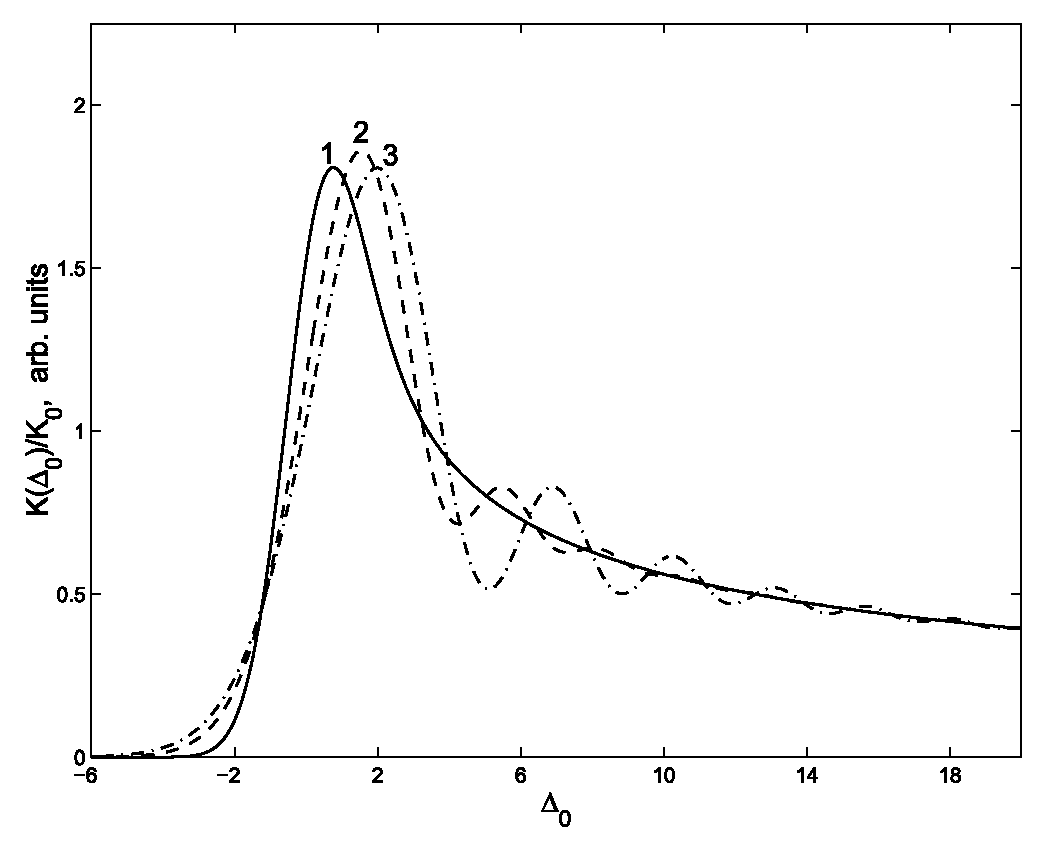
\includegraphics [scale=0.8] {fig_2_2_1}
	\caption{Частотная зависимость первого пика магнетопоглощения в режиме магнитоинфракрасного резонанса. Кривые 1, 2, 3 получены соответственно для $a=0$; $a=0.4$; $a=0.8$.} 
	\label{img:fig_2_2_1} 
\end{figure}

\begin{figure}[!h] 
	\center
	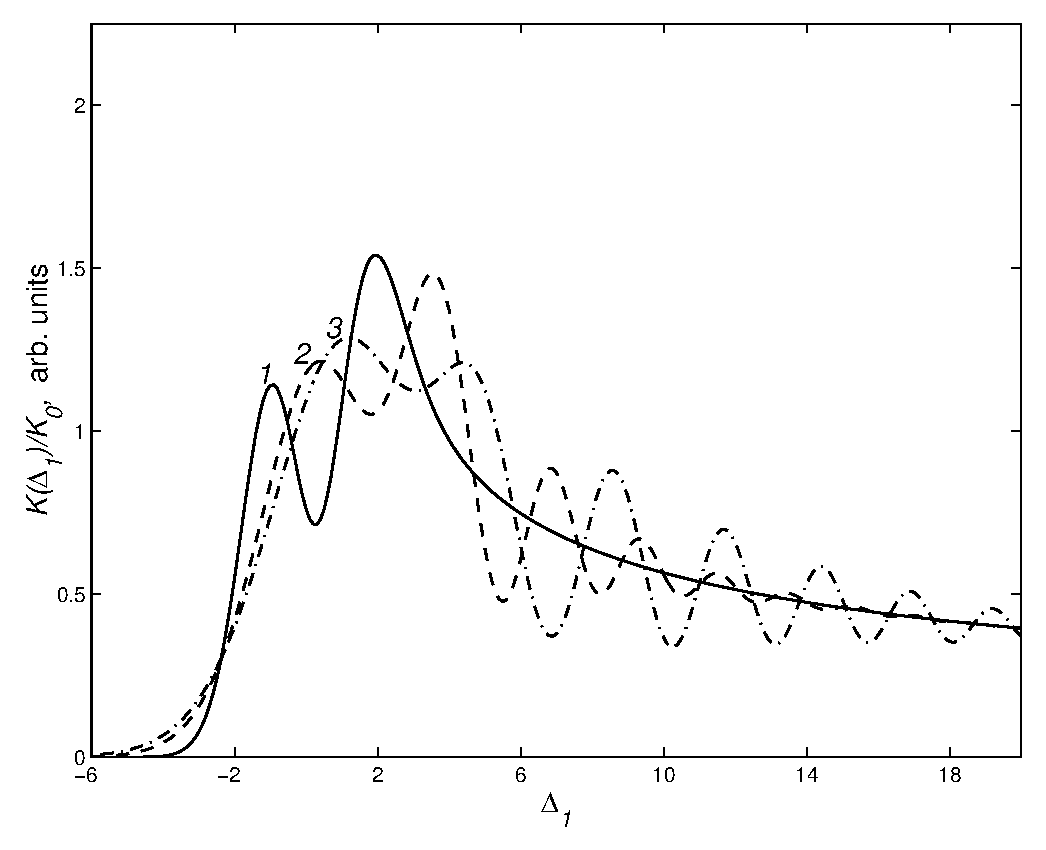
\includegraphics [scale=0.8] {fig_2_2_2}
	\caption{Частотная зависимость второго пика магнето-поглощения в режиме магнитоинфракрасного резонанса. Кривые 1, 2, 3 получены соответственно для $a=0$; $a=0.4$; $a=0.8$.} 
	\label{img:fig_2_2_2} 
\end{figure}

На рисунке~\ref{img:fig_2_2_1} представлены частотные зависимости линии магнетопоглощения в относительных единицах для $n=0$, т.е. для оптических переходов между нижайшими уровнями Ландау валентной зоны и зоны проводимости при различных значениях постоянного электрического поля. Кривые 1, 2, 3 получены соответственно для $a=0$, $a=0.4$, $a=0.8$.

Из представленных результатов видно, что с ростом напряженности электрического поля первый пик магнетопоглощения смещается, и в высокочастотной области возникают осцилляции коэффициента поглощения света. При переходе электрона на первый уровень Ландау (в формуле \eqref{eq:22_30} $n=1$) частотная зависимость второго пика магнетопоглощения описывается двумя пиками, причем величина длинноволнового пика меньше величины пика в высокочастотной области спектра (рисунок~\ref{img:fig_2_2_2}, кривая 1 получена при $a=0$). С ростом напряженности однородного электрического поля величина коротковолнового пика уменьшается, и в высокочастотной области возникают характерные осцилляции коэффициента поглощения света (кривые 2, 3 на рисунке~\ref{img:fig_2_2_2} получены при $a=0.4$, $a=0.8$ соответственно). 

Теперь рассмотрим межзонное поглощение слабой электромагнитной волны в параболических квантовых ямах, в которых благодаря размерному квантованию возникают эквидистантные зоны проводимости и валентные зоны. Если электрическое поле линейно-поляризованного излучения направлено вдоль оси пространственного квантования, то инфракрасное лазерное излучение смешивает ближайшие эквидистантные зоны.

Вычислим коэффициент межзонного поглощения слабого света, когда частота лазерного излучения $\omega $ равна частоте размерного квантования $\omega_c $ в зоне проводимости (размерно-инфракрасный резонанс -- РИР), а напряженность $E$ постоянного электрического поля направлена параллельно поверхности параболической квантовой ямы (ПКЯ). Коэффициент поглощения света $K(\Omega )$ вычисляется так же, как это было сделано выше и с учетом тех же приближений принимает следующий вид: 
\begin{multline} \label{eq:22_40} 
K(\Omega )=K_0 \sum _{n} \, V_n^2 \times  \\
\times \left\{\frac{\pi }{2} +\int_0^{\infty } dt \exp \left(-\frac{x^2 }{2} \right)L_n \left(x^2 \right)\frac{\sin \left[x\left(\Delta_n -\delta x^2 \right)\right]}{x} \right\}
\end{multline} 
где 
\[\Delta_n =\frac{\hbar \Omega -E_g -\hbar \omega^* \left(n+{\tfrac{1}{2}} \right)}{\hbar \sqrt{\gamma } } ; \; \omega^* =\omega_c +\omega_v ;\] 
$\hbar \omega_v $~---~энергия размерного квантования в валентной зоне, $V_n $~---~матричный элемент волновых функций электрона в зоне проводимости и в валентной зоне для ПКЯ \cite{Sinyavskii2002}. В отсутствии постоянного электрического поля $(E=0)$ \eqref{eq:22_40} переходит в выражение для межзонного поглощения света в режиме РИР, полученного в \cite{Sinyavskii2002}. В частном случае 
\[V_0 =\mathop{\left(\lambda_c \lambda_v \right)}\nolimits^{{\tfrac{1}{4}} } \sqrt{\frac{2}{\lambda_c +\lambda_v } } ;\; \; V_1 =2\sqrt{2} \frac{\mathop{\left(\lambda_c \lambda_v \right)}\nolimits^{{\tfrac{3}{4}} } }{\mathop{\left(\lambda_c +\lambda_v \right)}\nolimits^{{\tfrac{3}{2}} } } ;\; \; \lambda_i =\frac{m_i \omega^i }{\hbar } (i=c,v).\] 
Для типичных параметров ПКЯ GaAs-AlGaAS $\lambda_c /\lambda_v =0.47$ ($m_c =0.06m_0 ,$ $m_v =0.4m_0 $). На рисунке~\ref{img:fig_2_2_3} приведена частотная зависимость коэффициента межзонного поглощения света (в относительных единицах) при переходе электрона из нулевого (первого $n=1$) размерно-квантованного состояния валентной зоны на нулевое $n=0$ (первое $n=1$) размерно-квантованное состояние зоны проводимости. Кривая 1 описывает частотную зависимость коэффициента поглощения в отсутствии постоянного электрического поля \cite{Sinyavskii2002}. Кривая 2 получена при $a=0.4$, кривая 3 при $a=0.8$. Из рисунка~\ref{img:fig_2_2_3} видно, что постоянное продольное электрическое поле существенным образом влияет на межзонный коэффициент поглощения света. При этом в электрическом поле возможно заметное поглощение в длинноволновой области спектра, а в высокочастотной области поглощение света определяется характерной осцилляционной зависимостью от частоты. С ростом напряженности постоянного электрического поля осцилляции становятся наиболее отчетливыми. 
\begin{figure}[!h] 
	\center
	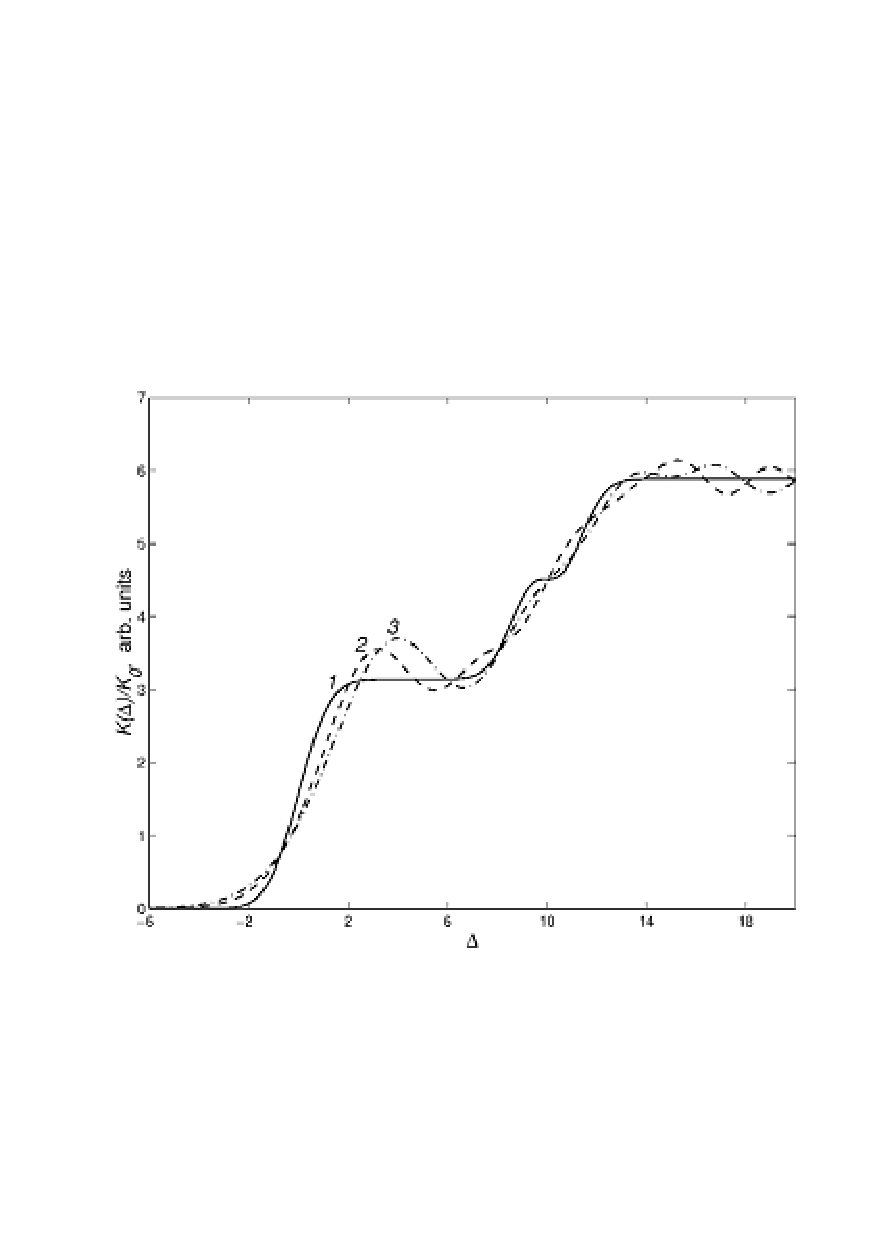
\includegraphics [scale=0.8] {fig_2_2_3}
	\caption{Частотная зависимость межзонного поглощения света в режиме размерно-инфракрасного резонанса. Кривые 1, 2, 3 получены соответственно для $a=0$; $a=0.4$; $a=0.8$.} 
	\label{img:fig_2_2_3} 
\end{figure}


\section{Оптические свойства квантовых проволок в присутствии резонансного лазерного излучения} \label{sect2_3}

Теперь исследуем явления, связанные с МИКР и размерно-инфракрасным резонансом (РИР) в квантовой проволоке в однородном магнитом поле $\vect{B}$ $(\vect{B} \parallel OZ)$, направленном перпендикулярно оси исследуемой наноструктуры с учетом взаимодействия носителей с шероховатой поверхностью. Такие одномерные структуры интересны тем, что имеют особенности в плотности энергетических состояний на дне размерно-квантованных зон, приводящие к особенностям оптических свойств. Энергетический спектр электрона в параболической нанопроволоке известен \cite{Hashimzade2005}:
\[
E_{\alpha }=\frac{\hbar^2 k^2_x}{2m^*_e}+\hbar \Omega_e\left(n+\frac{1}{2}\right)+\hbar {\omega }_e\left(m+\frac{1}{2}\right)
\] 
\[
m^*_e=m_e{\left(\frac{\Omega_e}{\omega_e}\right)}^2,\;
\Omega_e={\left[{\omega }^2_e+{\omega_c}^2\right]}^{1/2},\;
\omega_c=\frac{eB}{m_ec\ }
\] 
$\hbar\omega_e$~--~энергия размерного квантования электрона массы $m_e$ в зоне проводимости, $\omega_c$~--~циклотронная частота. Аналогично можно записать энергию для электрона в валентной зоне.

\begin{figure}[!h] 
	\center
	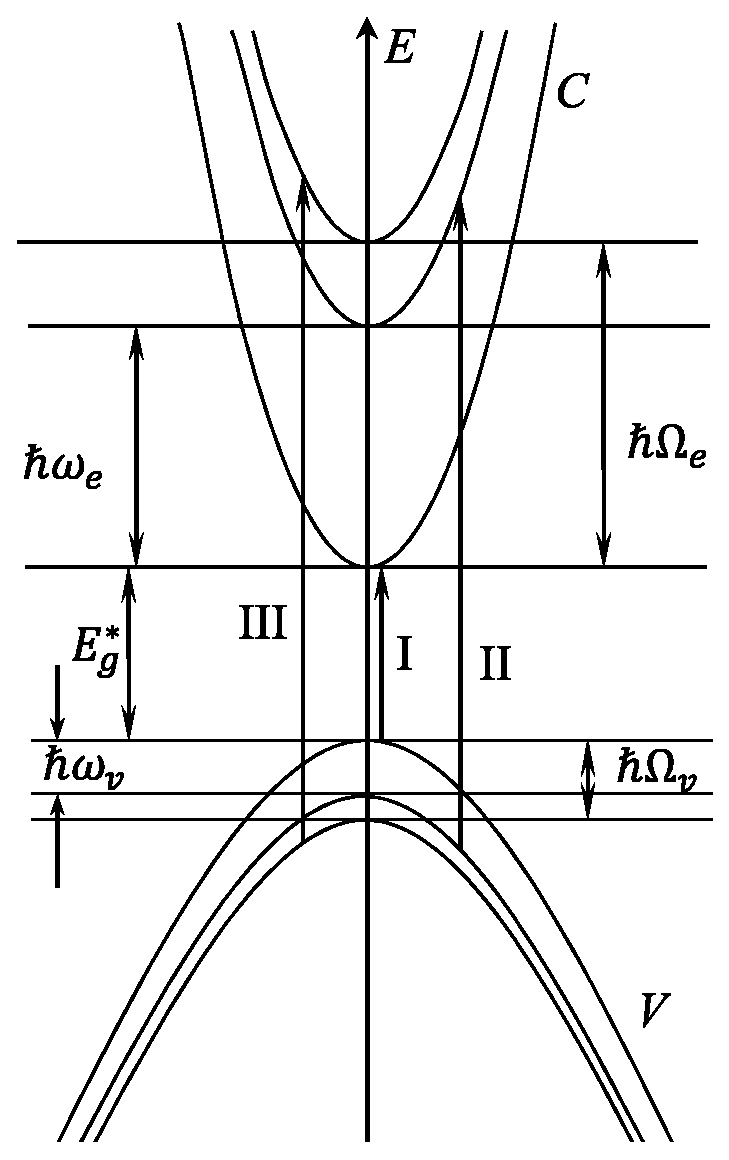
\includegraphics [scale=0.6] {fig_2_3_1}
	\caption{Схема энергетических зон полупроводниковой квантовой проволоки в поперечном магнитном поле и оптические переходы.} 
	\label{img:fig_2_3_1} 
\end{figure}

Будем исследовать оптические свойства полупроводниковых квантовых проволок (КП), схема энергетических зон которых изображена на рисунке~\ref{img:fig_2_3_1} $E^*_g$~---~ширина запрещенной зоны КП в магнитном поле, $\omega_v, \Omega_v$~---~соответственно частота размерного квантования и гибридная частота носителей в валентной зоне.

Вычислять коэффициент межзонного поглощения слабой электромагнитной волны в поле лазерного излучения, будем в случае, когда его частота $\omega_L$ равна $\omega_e$ частоте размерного квантования (РИР) или $\Omega_e$ (магнитно-инфракрасный резонанс). Так как для типичных полупроводниковых наноструктур эффективная масса электронов в зоне проводимости значительно меньше массы дырок ($m_e\ll m_v$), то взаимодействием интенсивного ИК излучения с электронами в валентной зоне в дальнейшем пренебрегаем ($\omega_e\gg \omega_v\ $).

Гамильтониан в представлении вторичного квантования для электронов в зоне проводимости в состоянии $\alpha $ в поле одномодового лазерного излучения поляризацией $\vect{\xi}$ записывается в следующем виде:
\begin{equation} \label{eq:23_10} 
\hat{H}=\sum_{\alpha } {\varepsilon_{\alpha } a^+_{\alpha } a_{\alpha }} + \hbar \omega_L b^+ b + {\left[\frac{2\pi \hbar e^2} {V \omega_L} \right]}^{\frac{1}{2}} {\sum_{\alpha \alpha_1}{\left|\frac{\vect{P}_{\alpha \alpha_1} \vect{\xi}}{m_e}\right|}}^2 a^+_{\alpha } a_{\alpha_1} (b^+ + b).
\end{equation}
Здесь $a^+_{\alpha }\ (a_{\alpha })$, $b^+ (b)$ -- операторы рождения (уничтожения) электронов в состоянии $\alpha $ и фотонов.

Расчет матричных элементов оператора импульса $\vect{P}_{\alpha\alpha_1}$ на волновых функциях параболической квантовой проволоки в поперечном магнитном поле \cite{Hashimzade2005} не представляет труда. В результате:
\begin{equation} \label{eq:23_20}
\begin{aligned}
&{\left| P^X_{\alpha \beta }\right|}^2=\frac{\delta^2}{\sqrt{\left(1+\delta^2\right)} }{\left|P^Y_{\alpha \beta }\right|}^2, \;
\delta =\frac{\omega_c}{\omega_e},\\
&\left| P^Y_{\alpha \beta }\right|^2=
\frac{m_e \sqrt{\left({1+\delta }^2\right)} \hbar\omega_e}{2} \left[  n \delta_{n,n_1+1} + (n+1) \delta_{n,n_1-1} \right]\delta_{k_x,k_x'}\delta_{m,m_1} , \\
&{\left| P^Z_{\alpha \beta }\right|}^2=\frac{m_e \hbar\omega_e}{2} \left[ m \delta_{m,m_1+1} + (m+1){\delta }_{m,m_1-1} \right]  \delta_{k_x,k_x'} \delta_{n,n_1}.
\end{aligned}
\end{equation}

Из выражения \eqref{eq:23_20} следует, что линейно X-поляризованная волна лазерного излучения (электромагнитная волна распространяется перпендикулярно оси нанопроволоки) в отсутствии магнитного поля $(\delta =0)$ не взаимодействует с зонными носителями. Согласно \eqref{eq:23_20} линейно Y-поляризованная волна (лазерное излучение распространяется вдоль оси квантовой проволоки) смешивает гибридные состояния $\left( \hbar\omega_L = \hbar\Omega_e \right) $, а Z-поляризованная волна (напряженность электрического поля лазерного излучения $\vect{E}\bot \vect{B}$) смешивает только размерно-квантованные состояния $ \left( \hbar\omega_L = \hbar\omega_e \right) $.

Расчет коэффициента межзонного поглощения слабой электромагнитной волны частоты $\Omega$ в поле резонансного лазерного излучения для квантовых проволок производился с использованием формулы Кубо \cite{Kubo1957a} и методики, развитой в \cite{Sinyavskii1974}. В результате при $\omega_L = \Omega_e$ (резонансный случай) для стабильно генерирующего ИК лазерного излучения Y-поляризации получаем:
\begin{multline} \label{eq:23_30}
K\left(\Omega\right)=K_0{\sum_{nm}{\left|\left\langle \alpha_c | \alpha_v \right\rangle \right|}}^2 
\int\limits_{-\infty }^{\infty }dk_x \int\limits_{-\infty }^{\infty }{dt \exp{\left( -a t^2 -\frac{\Gamma_0 }{\left|k_x\right|}|t| \right) }} L_n\left(2at^2 \right)\times\\
\times {\exp \left\{\frac{it}{\hbar }\left[\hbar \Omega-E^*_g-\frac{\hbar^2 k^2_x}{2\mu^*}-m\left(\hbar\omega_e+\hbar\omega_v\right)-n\left(\hbar\Omega_e + \hbar\Omega_v \right)\right]\right\}\ }
\end{multline}
\[
K_0=\frac{\hbar \Omega e^2}{4\mu^* E_g^* n_0 c s}, \;
a=\frac{e^2 E^2}{8 m_e \hbar\Omega_e},
\]
\[
\frac{1}{\mu^*}=\frac{1}{m^*_e}+\frac{1}{m^*_v},\;
m^*_v=m_v {\left(\frac{\Omega_v}{\omega_v}\right)}^2
\] 
$\left\langle \alpha_c | \alpha_v \right\rangle $~---~матричный элемент сглаженных волновых функций электрона в зоне проводимости и в валентной зоне, $L_n\left(z\right)$~---~полиномы Лаггера, $E$~---~напряженность электрического поля лазерного излучения, $s$~---~сечение квантовой проволоки. 

При записи \eqref{eq:23_30} учитывалось взаимодействие носителей с шероховатой поверхностью или с длинноволновыми акустическими фононами в приближении времени релаксации \cite{Khamidullin2002}. ${\Gamma_0}/{\left|k_x\right|}$~--~описывает вероятность рассеяния электронов в единицу времени или на шероховатой поверхности \eqref{eq:1_19}, \eqref{eq:1_20}  или упругое рассеяние на акустических фононах \cite{Khamidullin2006}.

Запишем коэффициент поглощения света, связанный с переходом электрона из нижайшей валентной зоны $(m=n=0)$ в нижайшую размерно-квантованную зону проводимости $(n=m=0)$. (Оптический переход I на рисунке~\ref{img:fig_2_3_1}) Интегрирование по $t$ в  \eqref{eq:23_30} проводится точно, в результате, после замены
\[
\frac{{\hbar }^2 k^2_x}{2\mu^*}=\hbar {\omega }_fx^2, \left(\omega^3_f = \frac{\hbar \gamma^2_0}{2\mu^*}\right)
\] 
соотношение  \eqref{eq:23_30} записывается в виде $\left(L_0\left(z\right)=1\right)$:
\begin{equation} \label{eq:23_40}
K\left(\Omega\right)=K_0\sum_{nm}{ {\lvert\langle \alpha_c | \alpha_v \rangle\rvert}^2 {\left[\frac{8\pi \mu^*\omega_f}{\hbar a}\right]}^{\frac{1}{2}} \mathrm{Re} \int\limits_0^\infty {dx e^{f^2\left(x\right)}\left[1-\Phi \left(f\left(x\right)\right)\right]}}
\end{equation}
\[
\Phi \left(z\right)=\frac{2}{\sqrt{\pi}}\int\limits_0^z {e^{-\tau^2}}d\tau ,
\] 
\[
f\left(x\right)={\left(\frac{\omega^2_f}{4a}\right)}^{\frac{1}{2}}\frac{1}{x}\left[1-ix\left(\frac{\Delta }{\hbar \omega_f}-x^2\right)\right],\; \Delta =\hbar \Omega-E^*_g .
\] 

В отсутствии лазерного излучения $(a=0)$ из \eqref{eq:23_40} при $\omega^2_f / 4a \gg 1$ можно получить выражение для коэффициента межзонного поглощения света в нанопроволоках в однородном магнитном поле \cite{Kostyukevich2015}. Если же $\omega^2_f / 4a \ll 1$, то форма линии межзонного поглощения света (высота, полуширина) полностью определяется интенсивностью лазерного излучения, и коэффициент поглощения света согласно \eqref{eq:23_40} записывается следующим образом 
\begin{equation} \label{eq:23_50}
K\left(\Omega\right)=K_0{\lvert\langle \alpha_c | \alpha_v \rangle\rvert}^2 {\left[\frac{8\pi \mu^*}{\hbar^2a}\right]}^{\frac{1}{2}} \exp{\left( -\frac{\Delta^2}{4a\hbar^2}\right) } \int\limits_0^\infty {dx \exp{\left( -\frac{x^4}{4a \hbar^2}+\frac{\Delta x^2}{2a \hbar^2}\right) }}
\end{equation}
После интегрирования по $x$ выражение \eqref{eq:23_50} примет вид:
\begin{equation} \label{eq:23_60}
K(\Omega)=K_0 {\lvert\langle \alpha_c | \alpha_v \rangle\rvert}^2
{\left[\frac{\pi {\mu }^*\left|\Delta \right|}{{\hbar }^2a}\right]}^{\frac{1}{2}}
\begin{cases}
e^{-z} \mathrm{K}_{1/4}(z), \Delta \le 0 \\ 
\frac{\pi }{\sqrt{2}}e^{-z}[\mathrm{I}_{{1}/{4}}\left(z\right)+\mathrm{I}_{-1/4}\left(z\right)], \Delta >0
\end{cases}
\end{equation}
\[
z=\frac{\Delta^2}{8a\hbar^2}=\frac{1}{2}\left(\frac{\Delta}{\hbar\omega_f} \right)^2 \left(\frac{\omega_f^2}{4a} \right),
\]
$\mathrm{K}_v\left(z\right)$~---~функция Макдональда, $\mathrm{I}_v\left(z\right)$~---~модифицированная функция Бесселя.

\begin{figure}[!h] 
	\center
	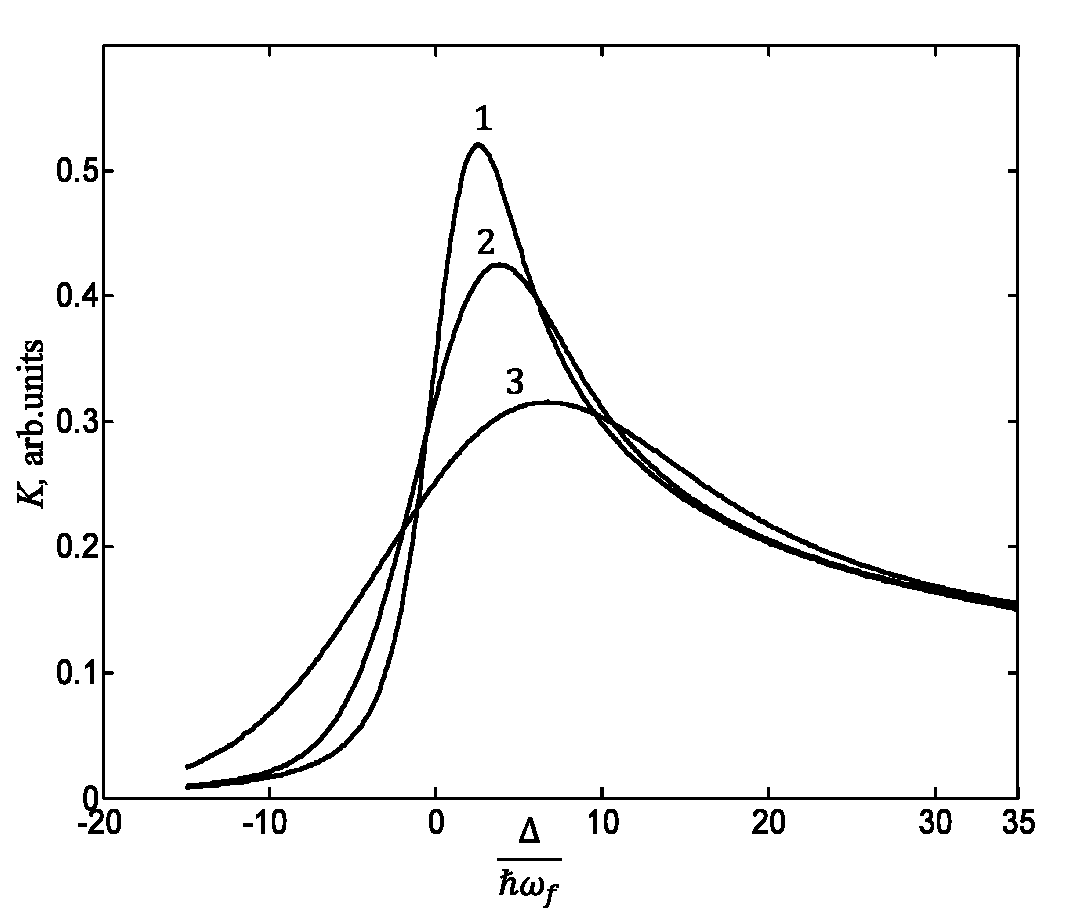
\includegraphics [scale=0.8] {fig_2_3_2}
	\caption{Зависимость первого пика межзонного поглощения света (в относительных единицах) от ${\Delta }/{\hbar {\omega }_f}$. Кривые 1, 2, 3 вычислены для $\xi =0.25,\; 0.05,\; 0.01$ соответсвенно.} 
	\label{img:fig_2_3_2} 
\end{figure}

На рисунке~\ref{img:fig_2_3_2} представлена частотная зависимость коэффициента поглощения света (в относительных единицах) при различных значениях интенсивности лазерного излучения. Кривые 1, 2, 3 получены соответственно при $\xi =0.25,\ 0.05,\ 0.01$ $\left(\xi =\omega^2_f / 4a \right)$. Как следует из рисунка~\ref{img:fig_2_3_2}, с ростом интенсивности ИК излучения ($\xi $ уменьшается при фиксированном значении $\omega_f$) форма линии поглощения изменяется: величина максимума поглощения уменьшается, а полуширина увеличивается. Заметим, что уже при $\xi \le 1$ коэффициент межзонного поглощения света полностью определяется интенсивностью ИК лазерного излучения.

Рассмотрим межзонное поглощение света в области второго пика магнетопоглощения (оптический переход II на рисунке~\ref{img:fig_2_3_1}) при $\omega_L=\Omega_e$ (магнито-инфракрасный резонанс). В этом случае коэффициент поглощения света согласно \eqref{eq:23_30} при $m=0$, $n=1$ $\left( L_1\left(2at^2\right)=1-2at^2 \right) $ принимает следующий вид:
\begin{multline} \label{eq:23_70}
K\left(\Omega\right)=K_0 {\left|\left\langle \widetilde{\alpha }_c |\widetilde{\alpha }_v\right\rangle \right|}^2 4{\left[\frac{2{\mu }^*{\omega }_f}{\hbar a}\right]}^{\frac{1}{2}}\times\\
\times Re\int\limits^{\infty }_0 {dx} f(x)\left\{-\sqrt{\pi }f\left(x\right)e^{f^2\left(x\right)}\left[1-\Phi \left(f\left(x\right)\right)\right]+1\right\}
\end{multline} 
 
При $\xi ={{\omega }^2_f}/{4a}\gg 1$ (лазерное излучение отсутствует) из \eqref{eq:23_70} следует выражение для коэффициента поглощения слабой электромагнитной волны, полученное в \cite{Kostyukevich2015}. При $\xi <1$ (форма линии поглощения определяется интенсивностью резонансного ИК излучения) получено:
\begin{multline} \label{eq:23_80}
K\left(\Omega\right)=K_0{\left|\left\langle \widetilde{\alpha }_c |\widetilde{\alpha }_v\right\rangle \right|}^2 \pi z{\left[\frac{2^* \pi }{\hbar }{\left(\frac{8z}{a}\right)}^{1/2}\right]}^{1/2}e^{-z}\times\\
\times \left\{-\left[I_{3/4}\left(z\right)+\mathrm{sign}(\Delta) I_{-3/4}\left(z\right)\right]+\left(1+\frac{1}{4z}\right)\left[(I_{-1/4}\left(z\right)+ \mathrm{sign}(\Delta)  I_{1/4}\left(z\right)\right]\right\}
\end{multline}
\[
\mathrm{sign}(\Delta) = \begin{cases}
1,&\Delta >0 \\ 
-1,&\Delta <0
\end{cases}
\] 
$\left\langle \widetilde{\alpha }_c |\widetilde{\alpha }_v \right\rangle$ --- матричный элемент сглаженных волновых функций носителей в возбужденном состоянии валентной зоны ($m=0$, $n=1$) и в первом возбужденном состоянии размерно-квантованной зоны проводимости.

\begin{figure}[!h] 
	\center
	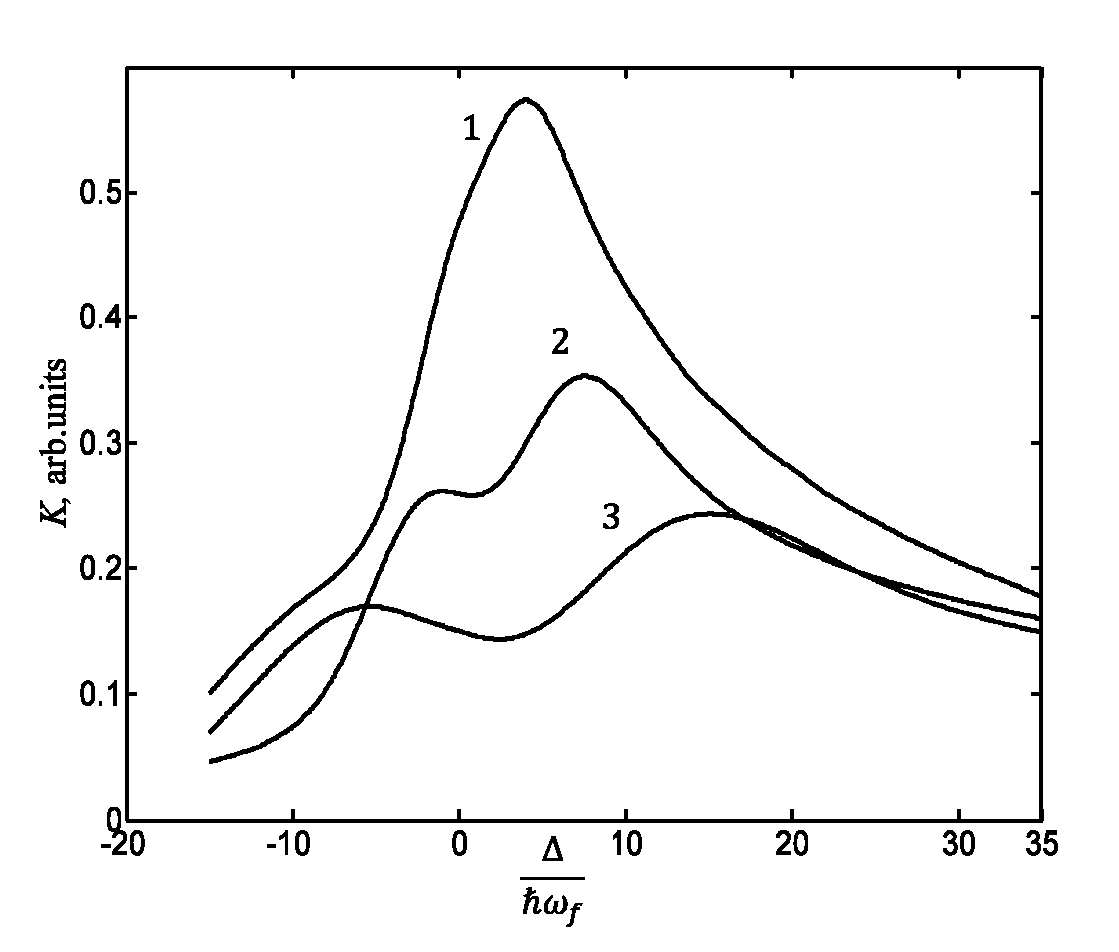
\includegraphics [scale=0.8] {fig_2_3_3}
	\caption{Зависимость второго пика магнетопоглощения (в относительных единицах) от ${\Delta }/{\hbar {\omega }_f}$ при различных значениях интенсивности резонансного $\left({\omega }_L=\Omega_e\right)$ лазерного излучения. Кривые 1, 2, 3 вычислены для $\xi=0.25,\; 0.05,\; 0.01$ соответсвенно.} 
	\label{img:fig_2_3_3} 
\end{figure}

На рисунке~\ref{img:fig_2_3_3} приведена частотная зависимость второго пика магнетопоглощения при различных значениях $\xi $. Кривые 1, 2, 3 вычислены при $\xi =0.25,\ \ 0.05,\ \ 0.01$ соответсвенно. Как следует из рисунка с ростом напряженности $E$ электрического поля пик магнетопоглощения деформируется и при $\xi \ll 1$ расщепляется на два пика. При этом расстояние между ними и их полуширина увеличивается. Расщепление второго пика поглощения связано с тем, что при $\omega_L=\Omega_e$ возбужденное гибридное состояние $(n=1)$ двукратно вырождено, и при взаимодействии с ИК лазерным излучением оно расщепляется. Эта ситуация близка к двойному оптическому резонансу (ДОР) на межзонных переходах в объемных материалах \cite{Perlin1970}.

Заметим, что $n$-пик магнетопоглощения расщепляется на $n$ пиков. Если рассматривать случай $z$-поляризованной электромагнитной волны лазерного излучения, когда $\omega_L=\omega_e$ (размерно-инфракрасный резонанс), то частотная зависимость коэффициента межзонного поглощения света (оптический переход III на рисунке~\ref{img:fig_2_3_1}) качественно не отличается от частотной зависимости, приведенной на рисунке~\ref{img:fig_2_3_2} и на рисунке~\ref{img:fig_2_3_3}.

Пусть при некотором значении напряженности электрического поля $E_c$ интенсивной электромагнитной волны вклад лазерного излучения в полуширину магнетоосцилляций примерно такой же как вклад, определяемый рассеянием носителей на шероховатой поверхности $(\xi =1)$. Естественно при $E_c<E$ форма линии межзонного поглощения слабой электромагнитной волны полностью определяется внешней лазерной подсветкой. Для типичных параметров полупроводниковой нанопроволоки $m_e=0.06m_0$, $m_v=0.4m_0$, $\sqrt[3]{\gamma_0}=20\ \AA $ (такое значение $\sqrt[3]{\gamma_0}$ хорошо описывает большие значения подвижности $\mu \propto 10^4\ \frac{cm^2}{V\cdot s}$, характерные для квантовых проволок) при $R_0=10^3\ \AA $, $E_c= 7\ \frac{V}{cm}$ для лазера $\mathrm{H_2 O}$ $\left(\hbar {\omega }_L=0.044\ eV\right)$. Следовательно, резонансное лазерное излучение заметно влияет на частотную зависимость межзонного поглощения света при небольших, вполне экспериментально доступных значений интенсивности ИК- лазерного излучения.
